\documentclass{article}

\usepackage[T1]{fontenc}
\usepackage{amsmath}
\usepackage{float}
\usepackage{longtable}
\usepackage{xcolor}
\usepackage{listings}
\usepackage{graphicx}
\usepackage{hyperref}
\usepackage{ragged2e}
\usepackage[a4paper,left=1.5cm,right=1.5cm]{geometry}

\newcommand\Que[2]{%
   \begin{samepage}
   \leavevmode\par
   \noindent
   Q.#1 --- #2\par\vspace{10pt}\hrule\vspace{10pt}
   \end{samepage}}

\newenvironment{ans}
   {\fbox{Answer}\begin{quote}\nopagebreak}
   {\end{quote}}
%
\newcommand\Refer[1]{
   \begin{center}
      {\small\textit{Reference:} \url{#1}}
   \end{center}
}%

\newcommand\ie{\emph{i.e.}}
\newcommand\INFOCOLSIZE{13em}

% Define Gruvbox colors
\definecolor{gruvboxbg}{HTML}{282828}
\definecolor{gruvboxfg}{HTML}{ebdbb2}
\definecolor{gruvboxgray}{HTML}{a89984}
\definecolor{gruvboxred}{HTML}{cc241d}
\definecolor{gruvboxgreen}{HTML}{98971a}
\definecolor{gruvboxyellow}{HTML}{d79921}
\definecolor{gruvboxblue}{HTML}{458588}
\definecolor{gruvboxpurple}{HTML}{b16286}
\definecolor{gruvboxaqua}{HTML}{689d6a}
\definecolor{gruvboxorange}{HTML}{d65d0e}

% Define Gruvbox-themed lstlisting environment
\lstdefinestyle{gruvboxstyle}{
  backgroundcolor=\color{gruvboxbg},
  basicstyle=\color{gruvboxfg}\ttfamily,
  keywordstyle=\color{gruvboxblue},
  commentstyle=\color{gruvboxgray},
  stringstyle=\color{gruvboxgreen},
  numberstyle=\tiny\color{gruvboxorange},
  identifierstyle=\color{gruvboxaqua},
  emphstyle=\color{gruvboxyellow},
  rulecolor=\color{gruvboxbg},
  frame=single,
  framerule=0pt,
  showstringspaces=false,
  breaklines=true,
  tabsize=2,
  numbers=left,
  numbersep=5pt,
}

% Define Gruvbox-themed lstlisting environment with caption and label
\lstnewenvironment{gruvboxlisting}[1][]
{
  \lstset{style=gruvboxstyle, #1}
}
{}
%

% Define a custom note environment
\newenvironment{note}{%
    \begin{quote}
    \textbf{Note:}%
}{%
    \end{quote}%
}


\RaggedRight

\begin{document}

\Que{1}{Configuration of the device group can best be understood
   in terms of what is happening ``under the hood'' (\ie{},
   beneath the surface, or behind the interface which the GUI
   provides). Describe the activities ``under the hood'' in
terms which you have learnt in your study of the OSI 7-layer
model.}

\begin{ans}
So, firstly, it is critical to notice that this completely
depends on what Ostinato does ``under the hood''. Specifically,
I would like to point out that Ostinato itself is an application
running in a Linux virtual machine which is virtually connected
to a docker container on the same machine. This of course
introduces another level of complexity which I do not believe is
feasible to consider here.

Also, I believe it is also not feasible to describe what
Ostinato precisely does internally as it requires an in depth
knowledge of the Ostinato codebase.

Having said this, I will restrict myself to a very shallow
explanation.

The two main OSI layers which concern the creation of device
groups are the Data Link (2nd) Layer and the Network (3rd)
Layer.

When we create a device group we are forced to give that device
group a base MAC (Media Access Control) address. We have to pick
also the number of devices which the device group will have. In
the case that there are more than one devices, Ostinato will
give the rest of the devices MAC addresses based on an address
offset which we specify. The MAC addresses are then used by
Ostinato to distinguish between these virtual devices at layer
2.

\begin{note}
The uniqueness of the MAC addresses used is responsibility of
the individual using Ostinato, although Ostinato seems to
provide random MAC address which are unlikely to be already in
use.
\end{note}

After we provide MAC addresses to the devices in the device
group we also have the option of choosing an Internet Protocol
(IP) version and provide a base IP address and an address offset
to give each device a different IP address. This essentially
sets up the virtual devices for layer 3 functionality.

I think the above is a sufficient answer as delving into the
actual details of how these things are implemented is not
trivial and would require an incredibly large amount of work.
\end{ans}

\newpage

\Que{2.1}{Count the number of packets that you have captured and
compare this with the setting in the stream configured on the
packet generator.}

\begin{ans}
\begin{center}
   \begin{longtable}{|l|l|l|l|l|l|p{\INFOCOLSIZE}|}
\caption{Wireshark ICMP capture for Question 2.1.}
\label{longtable:wireshark-cap-q2.1}\\
\hline 
\multicolumn{1}{|c|}{\textbf{No.}}&
\multicolumn{1}{c|}{\textbf{Time}}&
\multicolumn{1}{c|}{\textbf{Source}}&
\multicolumn{1}{c|}{\textbf{Destination}}&
\multicolumn{1}{c|}{\textbf{Protocol}}&
\multicolumn{1}{c|}{\textbf{Length}}&
\multicolumn{1}{c|}{\textbf{Info}}\\
\hline 
\endfirsthead

\multicolumn{7}{c}{\tablename\ \thetable{} -- continued from previous page}\\
\hline
\multicolumn{1}{|c|}{\textbf{No.}}&
\multicolumn{1}{c|}{\textbf{Time}}&
\multicolumn{1}{c|}{\textbf{Source}}&
\multicolumn{1}{c|}{\textbf{Destination}}&
\multicolumn{1}{c|}{\textbf{Protocol}}&
\multicolumn{1}{c|}{\textbf{Length}}&
\multicolumn{1}{c|}{\textbf{Info}}\\
\hline 
\endhead

\hline
\multicolumn{7}{|c|}{{continued on next page}}\\
\hline
\endfoot

\hline
\hline
\endlastfoot

486 & 4617.638757 & 192.168.0.10 & 192.168.0.1 & ICMP & 60 & Echo (ping)
request id=0x04d2, seq=0/0, ttl=127 (reply in 487) \\
487 & 4617.638893 & 192.168.0.1 & 192.168.0.10 & ICMP & 60 & Echo (ping)
reply id=0x04d2, seq=0/0, ttl=64 (request in 486) \\
488 & 4618.638764 & 192.168.0.10 & 192.168.0.1 & ICMP & 60 & Echo (ping)
request id=0x04d2, seq=0/0, ttl=127 (reply in 489) \\
489 & 4618.638848 & 192.168.0.1 & 192.168.0.10 & ICMP & 60 & Echo (ping)
reply id=0x04d2, seq=0/0, ttl=64 (request in 488) \\
490 & 4619.638761 & 192.168.0.10 & 192.168.0.1 & ICMP & 60 & Echo (ping)
request id=0x04d2, seq=0/0, ttl=127 (reply in 491) \\
491 & 4619.638880 & 192.168.0.1 & 192.168.0.10 & ICMP & 60 & Echo (ping)
reply id=0x04d2, seq=0/0, ttl=64 (request in 490) \\
492 & 4620.638772 & 192.168.0.10 & 192.168.0.1 & ICMP & 60 & Echo (ping)
request id=0x04d2, seq=0/0, ttl=127 (reply in 493) \\
493 & 4620.638890 & 192.168.0.1 & 192.168.0.10 & ICMP & 60 & Echo (ping)
reply id=0x04d2, seq=0/0, ttl=64 (request in 492) \\
494 & 4621.638731 & 192.168.0.10 & 192.168.0.1 & ICMP & 60 & Echo (ping)
request id=0x04d2, seq=0/0, ttl=127 (reply in 495) \\
495 & 4621.638861 & 192.168.0.1 & 192.168.0.10 & ICMP & 60 & Echo (ping)
reply id=0x04d2, seq=0/0, ttl=64 (request in 494) \\
496 & 4622.638714 & 192.168.0.10 & 192.168.0.1 & ICMP & 60 & Echo (ping)
request id=0x04d2, seq=0/0, ttl=127 (reply in 497) \\
497 & 4622.638914 & 192.168.0.1 & 192.168.0.10 & ICMP & 60 & Echo (ping)
reply id=0x04d2, seq=0/0, ttl=64 (request in 496) \\
500 & 4623.638729 & 192.168.0.10 & 192.168.0.1 & ICMP & 60 & Echo (ping)
request id=0x04d2, seq=0/0, ttl=127 (reply in 501) \\
501 & 4623.638837 & 192.168.0.1 & 192.168.0.10 & ICMP & 60 & Echo (ping)
reply id=0x04d2, seq=0/0, ttl=64 (request in 500) \\
502 & 4624.638727 & 192.168.0.10 & 192.168.0.1 & ICMP & 60 & Echo (ping)
request id=0x04d2, seq=0/0, ttl=127 (reply in 503) \\
503 & 4624.638831 & 192.168.0.1 & 192.168.0.10 & ICMP & 60 & Echo (ping)
reply id=0x04d2, seq=0/0, ttl=64 (request in 502) \\
504 & 4625.638735 & 192.168.0.10 & 192.168.0.1 & ICMP & 60 & Echo (ping)
request id=0x04d2, seq=0/0, ttl=127 (reply in 505) \\
505 & 4625.638858 & 192.168.0.1 & 192.168.0.10 & ICMP & 60 & Echo (ping)
reply id=0x04d2, seq=0/0, ttl=64 (request in 504) \\
506 & 4626.638725 & 192.168.0.10 & 192.168.0.1 & ICMP & 60 & Echo (ping)
request id=0x04d2, seq=0/0, ttl=127 (reply in 507) \\
507 & 4626.638833 & 192.168.0.1 & 192.168.0.10 & ICMP & 60 & Echo (ping)
reply id=0x04d2, seq=0/0, ttl=64 (request in 506) \\
\end{longtable}
\end{center}

There are 20 ICMP packets. 10 requests and 10 replies.

\begin{figure}[H]
   \centering
   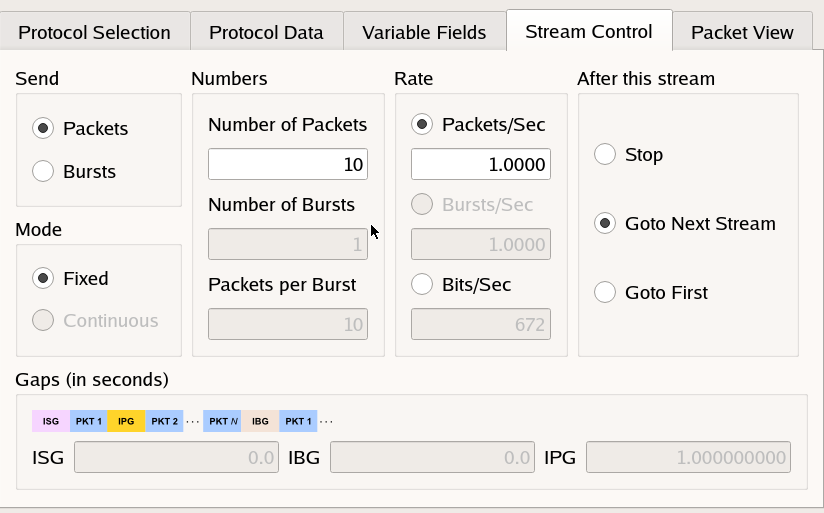
\includegraphics[width=10cm]{data/q2.1-stream-settings.png}
   \caption{The stream settings in Ostinato for Question 2.1.}
   \label{fig:stream-settings-q2.1}
\end{figure}

As can be seen in Figure \ref{fig:stream-settings-q2.1} the
number of packets, specifically requests, was precisely set to
10.

\end{ans}

\newpage

\Que{2.2}{Write down the numbers (leftmost column) of the packets that have been generated by:
\begin{itemize}
\item the packet generator
\item the DUT
\end{itemize}
}

\begin{ans}
The required values can be read off Table
\ref{longtable:wireshark-cap-q2.1}.

486, 488, 490, 492, 494, 496, 500, 502, 504 and 506 are the
numbers associated with the request packets generated by
Ostinato.

487, 489, 491, 493, 495, 497, 501, 503, 505 and 507 are the
numbers associated with the reply packets sent by the DUT.
\end{ans}

\Que{2.3}{Use your answer to 2.2 to find the average
inter-packet delay for the packets generated by the packet
generator.}
\begin{ans}

$$
\begin{aligned}
&\frac{
\begin{aligned}
&(4618.638764 - 4617.638757)
+(4619.638761 - 4618.638764)
+(4620.638772 - 4619.638761)\\
+\ &(4621.638731 - 4620.638772)
+(4622.638714 - 4621.638731)
+(4623.638729 - 4622.638714)\\
+\ &(4624.638727 - 4623.638729)
+(4625.638735 - 4624.638727)
+(4626.638725 - 4625.638735)
\end{aligned}
}{10 - 1}\\
=\ & 0.9999964444444535\ \text{seconds}\\
\approx\ & 1\ \text{seconds}
\end{aligned}
 $$

 The above computed value is the average inter-packet delay (in
 seconds). The approximate value, 1, is precisely what was set
 in the stream's settings, see Figure
 \ref{fig:stream-settings-q2.1}.

\begin{gruvboxlisting}[language=Python, caption={Python
   expression for calculating the inter-packet delay for
Question 2.3.}]
((4618.638764 - 4617.638757)
+(4619.638761 - 4618.638764)
+(4620.638772 - 4619.638761)
+(4621.638731 - 4620.638772)
+(4622.638714 - 4621.638731)
+(4623.638729 - 4622.638714)
+(4624.638727 - 4623.638729)
+(4625.638735 - 4624.638727)
+(4626.638725 - 4625.638735))/9
\end{gruvboxlisting}

\end{ans}

\newpage

\Que{3}{Repeat the exercises of question 2 with the new packet
rate (2 pkt/s).}

\begin{ans}
\begin{figure}[H]
   \centering
   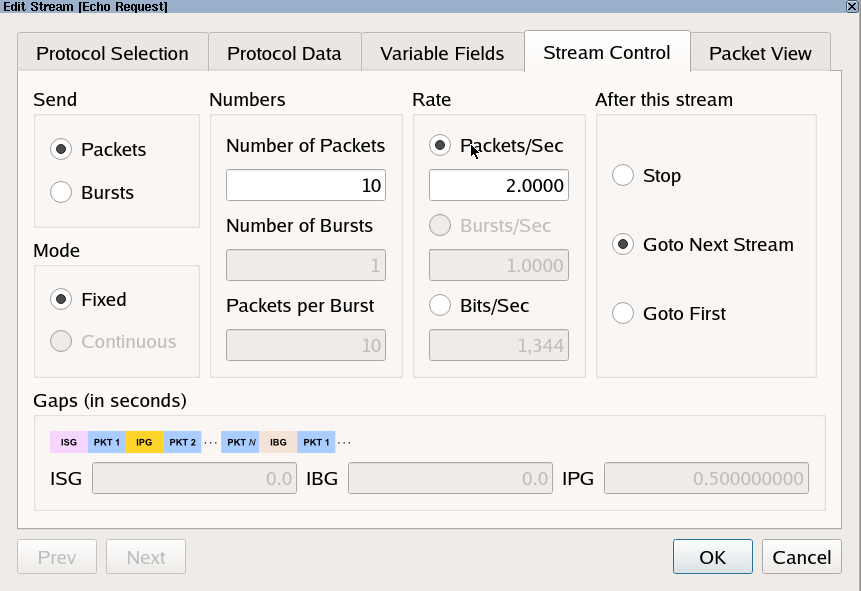
\includegraphics[width=10cm]{data/q3-stream-settings.png}
   \caption{The stream settings in Ostinato for Question 3}
   \label{fig:stream-settings-q3}
\end{figure}

\begin{center}
\begin{longtable}{|l|l|l|l|l|l|p{\INFOCOLSIZE}|}
\caption{Wireshark ICMP capture for Question 3.}
\label{longtable:wireshark-cap-q3}\\
\hline 
\multicolumn{1}{|c|}{\textbf{No.}}&
\multicolumn{1}{c|}{\textbf{Time}}&
\multicolumn{1}{c|}{\textbf{Source}}&
\multicolumn{1}{c|}{\textbf{Destination}}&
\multicolumn{1}{c|}{\textbf{Protocol}}&
\multicolumn{1}{c|}{\textbf{Length}}&
\multicolumn{1}{c|}{\textbf{Info}}\\
\hline 
\endfirsthead

\multicolumn{7}{c}{\tablename\ \thetable{} -- continued from previous page}\\
\hline
\multicolumn{1}{|c|}{\textbf{No.}}&
\multicolumn{1}{c|}{\textbf{Time}}&
\multicolumn{1}{c|}{\textbf{Source}}&
\multicolumn{1}{c|}{\textbf{Destination}}&
\multicolumn{1}{c|}{\textbf{Protocol}}&
\multicolumn{1}{c|}{\textbf{Length}}&
\multicolumn{1}{c|}{\textbf{Info}}\\
\hline 
\endhead

\hline
\multicolumn{7}{|c|}{{continued on next page}}\\
\hline
\endfoot

\hline
\hline
\endlastfoot

16 & 140.926179 & 192.168.0.10 & 192.168.0.1 & ICMP & 60 & Echo (ping)
request id=0x04d2, seq=0/0, ttl=127 (reply in 17) \\
17 & 140.926306 & 192.168.0.1 & 192.168.0.10 & ICMP & 60 & Echo (ping)
reply id=0x04d2, seq=0/0, ttl=64 (request in 16) \\
18 & 141.426171 & 192.168.0.10 & 192.168.0.1 & ICMP & 60 & Echo (ping)
request id=0x04d2, seq=0/0, ttl=127 (reply in 19) \\
19 & 141.426320 & 192.168.0.1 & 192.168.0.10 & ICMP & 60 & Echo (ping)
reply id=0x04d2, seq=0/0, ttl=64 (request in 18) \\
20 & 141.926165 & 192.168.0.10 & 192.168.0.1 & ICMP & 60 & Echo (ping)
request id=0x04d2, seq=0/0, ttl=127 (reply in 21) \\
21 & 141.926287 & 192.168.0.1 & 192.168.0.10 & ICMP & 60 & Echo (ping)
reply id=0x04d2, seq=0/0, ttl=64 (request in 20) \\
22 & 142.426145 & 192.168.0.10 & 192.168.0.1 & ICMP & 60 & Echo (ping)
request id=0x04d2, seq=0/0, ttl=127 (reply in 23) \\
23 & 142.426254 & 192.168.0.1 & 192.168.0.10 & ICMP & 60 & Echo (ping)
reply id=0x04d2, seq=0/0, ttl=64 (request in 22) \\
24 & 142.926106 & 192.168.0.10 & 192.168.0.1 & ICMP & 60 & Echo (ping)
request id=0x04d2, seq=0/0, ttl=127 (reply in 25) \\
25 & 142.926275 & 192.168.0.1 & 192.168.0.10 & ICMP & 60 & Echo (ping)
reply id=0x04d2, seq=0/0, ttl=64 (request in 24) \\
26 & 143.426150 & 192.168.0.10 & 192.168.0.1 & ICMP & 60 & Echo (ping)
request id=0x04d2, seq=0/0, ttl=127 (reply in 27) \\
27 & 143.426249 & 192.168.0.1 & 192.168.0.10 & ICMP & 60 & Echo (ping)
reply id=0x04d2, seq=0/0, ttl=64 (request in 26) \\
28 & 143.926104 & 192.168.0.10 & 192.168.0.1 & ICMP & 60 & Echo (ping)
request id=0x04d2, seq=0/0, ttl=127 (reply in 29) \\
29 & 143.926259 & 192.168.0.1 & 192.168.0.10 & ICMP & 60 & Echo (ping)
reply id=0x04d2, seq=0/0, ttl=64 (request in 28) \\
30 & 144.426138 & 192.168.0.10 & 192.168.0.1 & ICMP & 60 & Echo (ping)
request id=0x04d2, seq=0/0, ttl=127 (reply in 31) \\
31 & 144.426250 & 192.168.0.1 & 192.168.0.10 & ICMP & 60 & Echo (ping)
reply id=0x04d2, seq=0/0, ttl=64 (request in 30) \\
32 & 144.926075 & 192.168.0.10 & 192.168.0.1 & ICMP & 60 & Echo (ping)
request id=0x04d2, seq=0/0, ttl=127 (reply in 33) \\
33 & 144.926259 & 192.168.0.1 & 192.168.0.10 & ICMP & 60 & Echo (ping)
reply id=0x04d2, seq=0/0, ttl=64 (request in 32) \\
34 & 145.426128 & 192.168.0.10 & 192.168.0.1 & ICMP & 60 & Echo (ping)
request id=0x04d2, seq=0/0, ttl=127 (reply in 35) \\
35 & 145.426236 & 192.168.0.1 & 192.168.0.10 & ICMP & 60 & Echo (ping)
reply id=0x04d2, seq=0/0, ttl=64 (request in 34) \\
\end{longtable}
\end{center}

Again the number of packets in total is 20. 10 requests and 10
replies as specified in the stream's settings, see Figure
\ref{fig:stream-settings-q3}.

And from Table \ref{longtable:wireshark-cap-q3} we can get the
respective No. of the request and reply packets

The request packets are precisely numbers: 16, 18, 20, 22, 24,
26, 28, 30, 32, 34.

And the reply packets are precisely numbers: 17, 19, 21, 23, 25,
27, 29, 31, 33, 35.

Finally, the below computed value is the average inter-packet
delay (in seconds).

$$
\begin{aligned}
&\frac{
\begin{aligned}
&(141.426171 - 140.926179)
+(141.926165 - 141.426171)
+(142.426145 - 141.926165)\\
+\ &(142.926106 - 142.426145)
+(143.426150 - 142.926106)
+(143.926104 - 143.426150)\\
+\ &(144.426138 - 143.926104)
+(144.926075 - 144.426138)
+(145.426128 - 144.926075)
\end{aligned}
}{10 - 1}\\
=\ & 0.499994333333335\ \text{seconds}\\
\approx\ & 0.5\ \text{seconds}
\end{aligned}
$$

The approximate value, 0.5, is precisely what should be expected
since if two request are being sent per second, see Figure
\ref{fig:stream-settings-q3}, that would equate to a packer
every half a second which is precisely 0.5 seconds.

\newpage

\begin{gruvboxlisting}[language=Python,caption={Python
   expression for calculating the inter-packet delay for
Question 3.}]
((141.426171 - 140.926179)
+(141.926165 - 141.426171)
+(142.426145 - 141.926165)
+(142.926106 - 142.426145)
+(143.426150 - 142.926106)
+(143.926104 - 143.426150)
+(144.426138 - 143.926104)
+(144.926075 - 144.426138)
+(145.426128 - 144.926075))/9
\end{gruvboxlisting}
\end{ans}

\Que{4.1}{Expand the frame section and inspect it to find out
the number of bytes captured by Wireshark from the link (``bytes
on wire'').}

\begin{ans}
\begin{figure}[H]
   \centering
   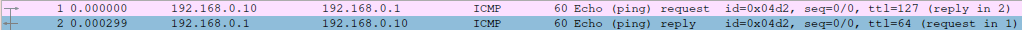
\includegraphics[width=16cm]{data/q4.1-packets-under-inspection.png}
   \caption{The packets under inspection for Question 4.1.}
\end{figure}

The info related to the request from the generator to the DUT is
provided below. Specifically, the information related to the
Ethernet II frame.

\begin{figure}[H]
   \centering
   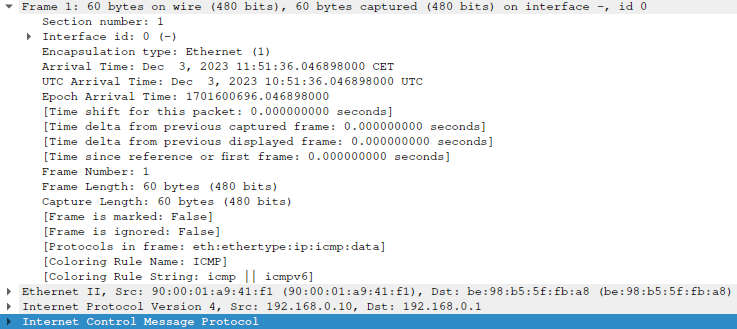
\includegraphics[width=16cm]{data/q4.1-request-info.png}
   \caption{The frame information of the request packet under
   insception for Question 4.1.}
\end{figure}

The number of bytes capture by Wireshark is exactly 60 bytes.
\end{ans}

\Que{4.2}{Search for the minimum length of an Ethernet packet,
and state it.}

\begin{ans}

\begin{figure}[H]
   \centering
   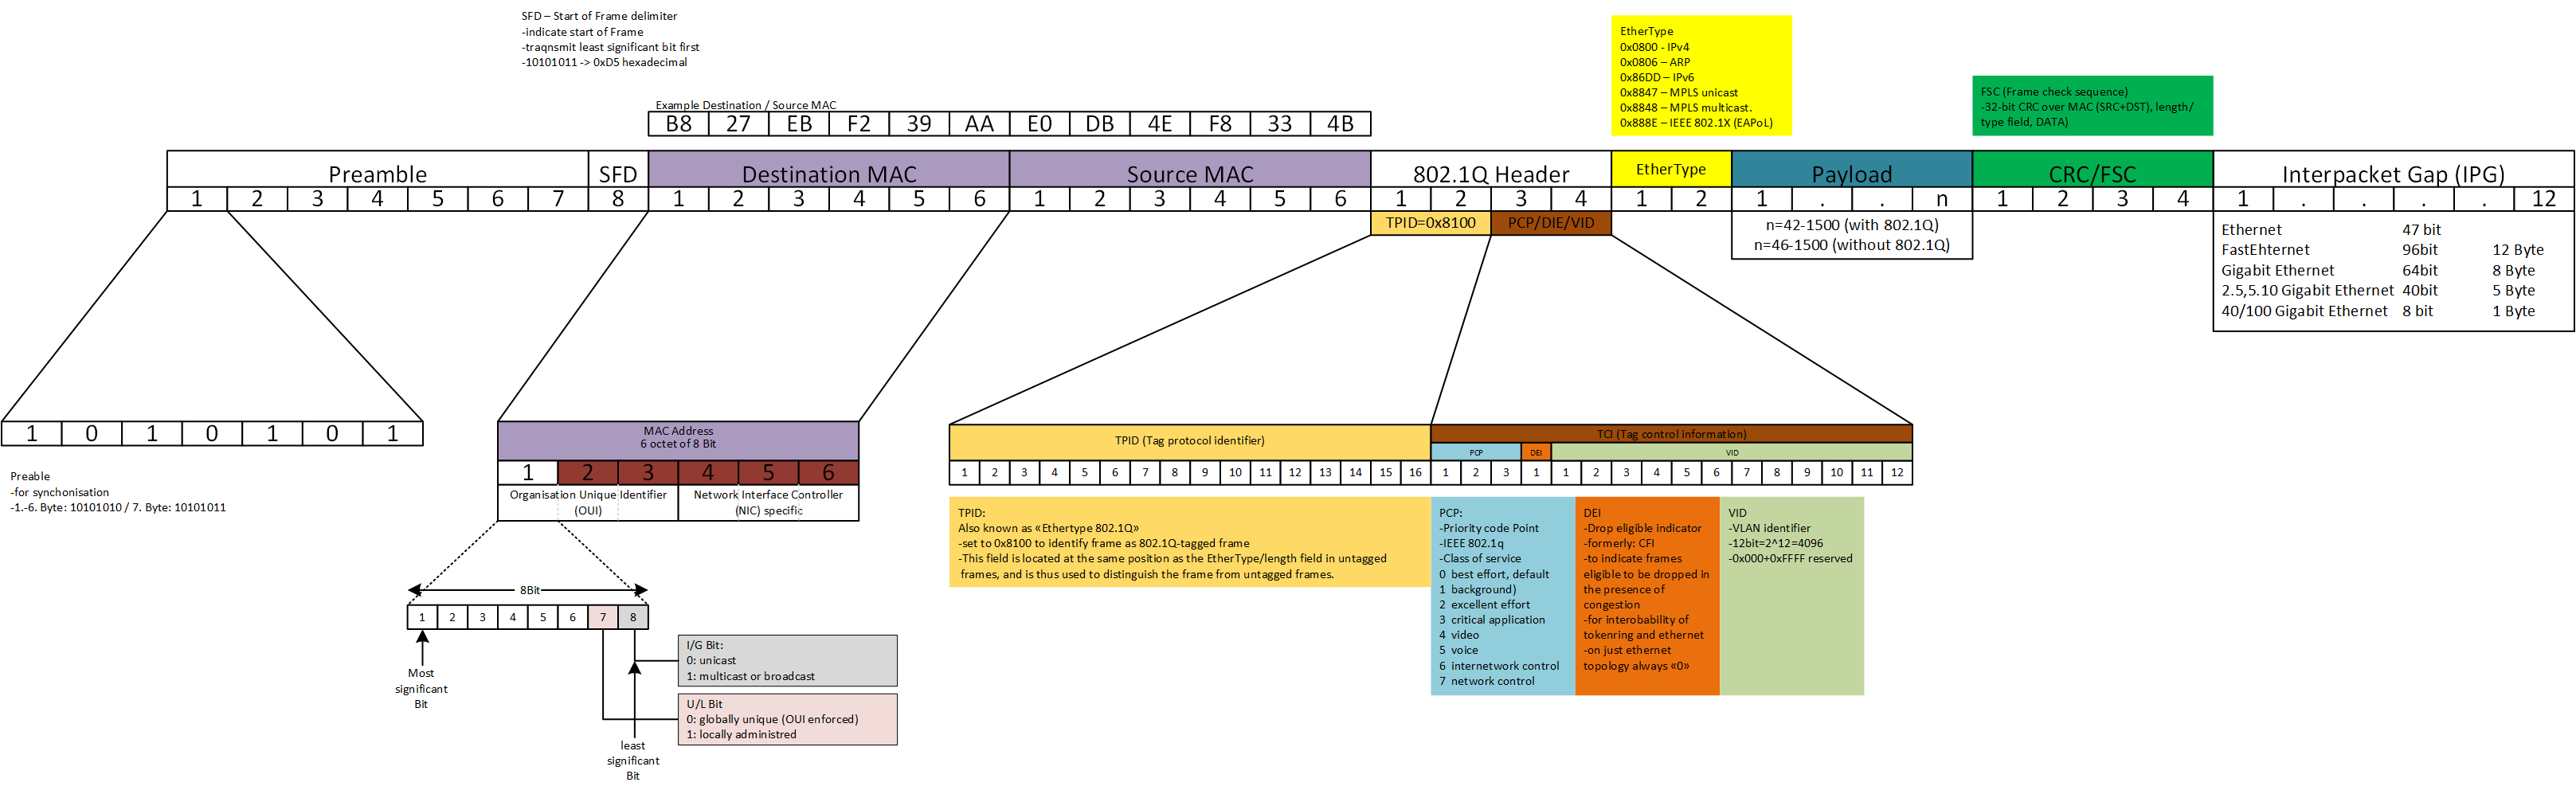
\includegraphics[width=16cm]{data/q4.2-ethernet-diagram.png}
   \caption{A diagram of the components of an Ethernet II frame.}
   \label{fig:eth2-frame}
\end{figure}

\Refer{https://upload.wikimedia.org/wikipedia/commons/7/72/Ethernet_Frame.png}

\begin{note}
There is a mistake in the graphic. ``CRC/FSC'' should be
``CRC/FCS'' and ``FSC (Frame check sequence)'' should be ``FCS
(Frame check sequence)''.
\end{note}

The minimum and maximum lengths can be derived from Figure
\ref{fig:eth2-frame}. Importantly, the preamble, SFD and
inter-pack gap are almost never exposed beyond layer 1.
Therefore, we shall not factor these into our calculation.

Hence, the Ethernet II frame at layer 2 consists of the
following segments:

\begin{itemize}
\item Destination MAC (6 octets);
\item Source MAC (6 octets);
\item 802.1Q Header (optional \& 4 octets);
\item EtherType (2 octets);
\item Payload (42 --- 1500 octets with 802.1Q \& 46 --- 1500
   octets without 802.1Q); and
\item CRC/FCS (4 octets).
\end{itemize}

Following this, the minimum length can be calculated follows:

$$
{\text{Frame}}_{\text{min}} = 6 + 6 + 2 + 46 + 4 = 64\ \text{octets}
$$

\begin{note}
In the case when there is no 802.1Q header, the total header and
payload lengths add up to 46. This is because the header length
is 0 and the payload has a minimum length of 46. In the other
case \ie{} when there is a 802.1Q header, the total header and
payload lengths also add up to 46. This is because the header
length is 4 and the payload length has a new minimum of 42,
since 4 have already been used by 802.1Q header. Hence, both
cases the sum of their lengths is identical.
\end{note}

Similarly, the maximum length is given by the following
calculation:

$$
{\text{Frame}}_{\text{max}} = 6 + 6 + 2 + 1500 + 4 = 1518\ \text{octets}
$$
\end{ans}

\Que{4.3}{How does the number of bytes captured (which you found
in (4.1)) compare with the minimum length of an Ethernet packet
(which you looked up in (4.2))? Can you explain the difference?}

\begin{ans}

\begin{figure}[H]
   \centering
   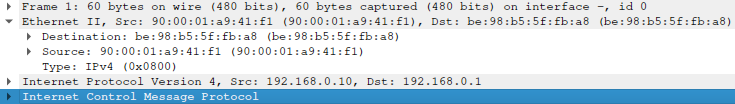
\includegraphics[width=14cm]{data/q4.3-ethernet-header.png}
   \caption{The Ethernet II header of the request packet under
   inspection for Question 4.1.}
   \label{fig:eth2-header-for-q4.3}
\end{figure}

The number of ``bytes on wire'' according to Wireshark, see
Figure \ref{fig:eth2-header-for-q4.3}, is precisely 60 bytes.
However, the minimum number of bytes is at least 64. This of
course, is a 4 byte discrepancy. 

To account for this discrepancy, notice that the Ethernet II
header does not contain an 802.1Q header. Hence, the payload is
allowed a minimum of 46 bytes. Additionally, all these 46 bytes
are used up by the ICMP request (including all IP overhead).

Hence, the Ethernet header and ICMP request sum up to 60 bytes.
This leaves only one option as to what the remaining 4 bytes can
they constitute the Cyclic Redundancy Check (CRC) or Frame Check
Sequence (FCS). In fact, according to Figure
\ref{fig:eth2-frame}, CRC field is exactly 4 bytes.

Furthermore, this conclusion is further supported by the below
referenced Wireshark forum discussion. One of the users exclaims
that ``bytes on wire'' is often more like ``bytes on wire
without CRC''. This is the case because most network drivers do
not provide the CRC to user space applications, instead invalid
packets are just immediately dropped.

\Refer{https://osqa-ask.wireshark.org/questions/1344/does-frame-length-include-also-crc-bytes}
\end{ans}

\Que{4.4}{Expand the Ethernet II section and write down the
source MAC address and the destination MAC address.}

\begin{ans}
Source MAC = \texttt{90:00:01:a9:41:f1}

Destination MAC = \texttt{be:98:b5:5f:fb:a8}

The above where taken from Figure \ref{fig:eth2-header-for-q4.3}.
\end{ans}

\newpage

\Que{4.5}{Look up the source MAC address in the device group
configured on the packet generator at the port group.}
\begin{ans}
\begin{figure}[H]
   \centering
   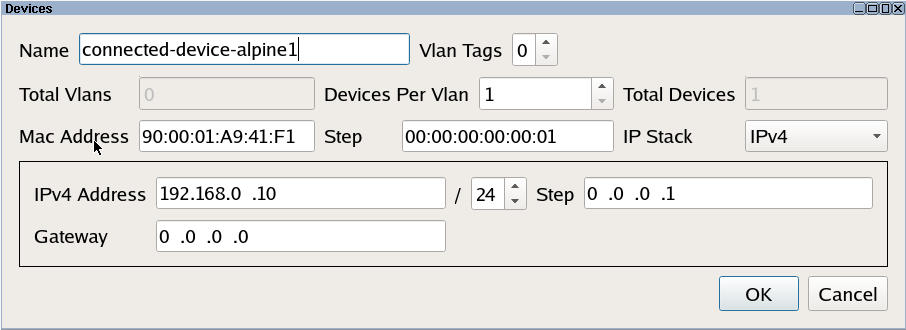
\includegraphics[width=14cm]{data/q4.5-device-group-config.png}
   \caption{The device group configuration in Ostinator for
   Question 4.5.}
   \label{fig:devic-config-q4.5}
\end{figure}
\begin{note}
	Since the device group contains as single device the
	base MAC address \ie{} \texttt{90:00:01:a9:41:f1} is used for that
	device.
\end{note}

As can be seen in Figure \ref{fig:devic-config-q4.5}, the device is given the MAC address \texttt{90:00:01:a9:41:f1}.
\end{ans}

\Que{4.6}{Compare what was found in 4.4 with what was found in
4.5.}
\begin{ans}
	\begin{note}
		Assuming that in the original question, 5.4 and 5.5 where
		meant to be 4.4 and 4.5 respectively.
	\end{note}
	
	As expected, the MAC address of the virtual device is
	identical to the source MAC Address in the packet. This is
	because the packet is a request packet \ie{} it
	was created by Ostinato.
	
	It is also critical to notice that the request is very much
	dependent on ARP (Address Resolution Protocol) to
	establish who has which MAC addresses.
\end{ans}

\Que{4.7}{Inspect the Ethernet II section and find the field in
that section which the receiver (the DUT) uses to identify the
layer 3 entity which is to receive the Ethernet frame's
payload.}
\begin{ans}
	In Question 4.2 the EtherType field is referenced. The EtherType field specifies what type of payload the Ethernet frame contains. The EtherType in the frame of interest is set to \texttt{0x0800}, see Figure \ref{fig:eth2-header-for-q4.3}. \texttt{0x0800} identifies the payload inside the frame as an IPv4 packet. This gives the DUT the required information to properly decode the contents of the payload.
\end{ans}

\Que{4.8}{Inspect the section below the Ethernet II section and:
\begin{itemize}
\item write down the source address and the destination address
   that you see in this underlying section;
\item compare the source address and the destination address
   with what you have set up in the stream named ``ICMP Echo
   Request Stream''.
\item Look up the field named ``Total length'' in this section
   and account for the difference between this number and the
   number you have found in 4.1.
\end{itemize}}

\begin{ans}
	\begin{figure}[H]
		\centering
		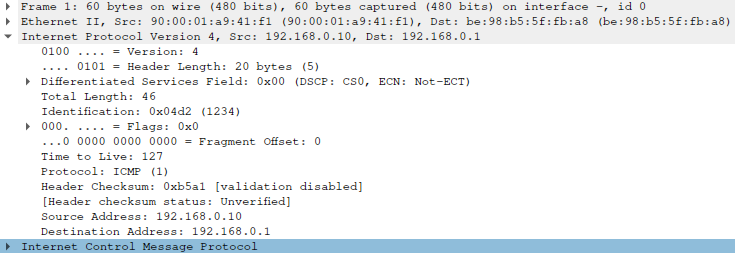
\includegraphics[width=14cm]{data/q4.8-ip-header.png}
		\caption{The IPv4 header of the request packet under
			inspection for Question 4.1.}
		\label{fig:ip-header-for-q4.8}
	\end{figure}
	
	Source IP Address = \texttt{192.168.0.10}
	
	Destination IP Address = \texttt{192.168.0.1}
	
	See Figure \ref{fig:ip-header-for-q4.8} to verify the above addresses.
	
	\begin{figure}[H]
		\centering
		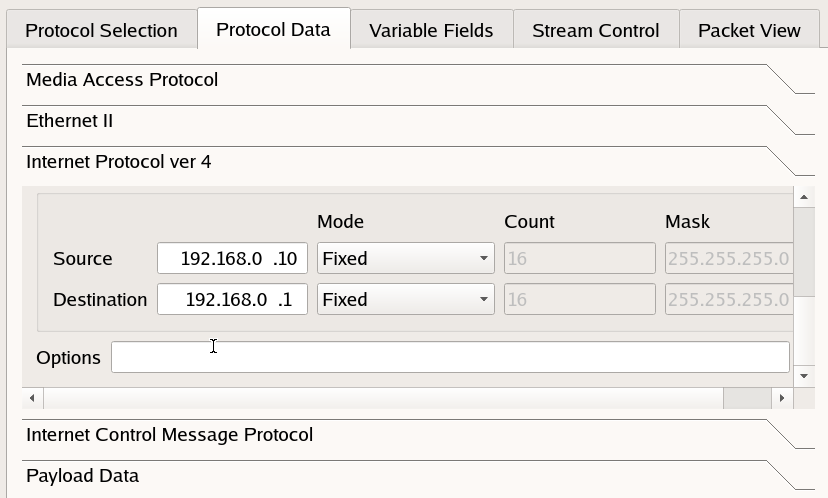
\includegraphics[width=14cm]{data/q4.8-stream-config.png}
		\caption{The stream's IPv4 configuration in Ostinato for Question 4.8.}
		\label{fig:stream-config-for-q4.8}
	\end{figure}
	
	Additionally, the Total Length is 46 bytes, again see Figure \ref{fig:ip-header-for-q4.8}. This is precisely
	what was described in Question 4.3. Again, the Ethernet header length is
	14 bytes, and $14 + 46 = 60$ bytes as expected.
	
	Additionally, 20 of the 46 bytes are the IPv4 Header Length whilst the remaining 26 bytes are the actual ICMP Request.
\end{ans}


\Que{5}{For each packet, state source and destination IPv4
address. Compare these latter two addresses with the IPv4
address bound to alpine-1 eth0, and justify the outcome of your
comparison.}

\begin{ans}
	\begin{figure}[H]
		\centering
		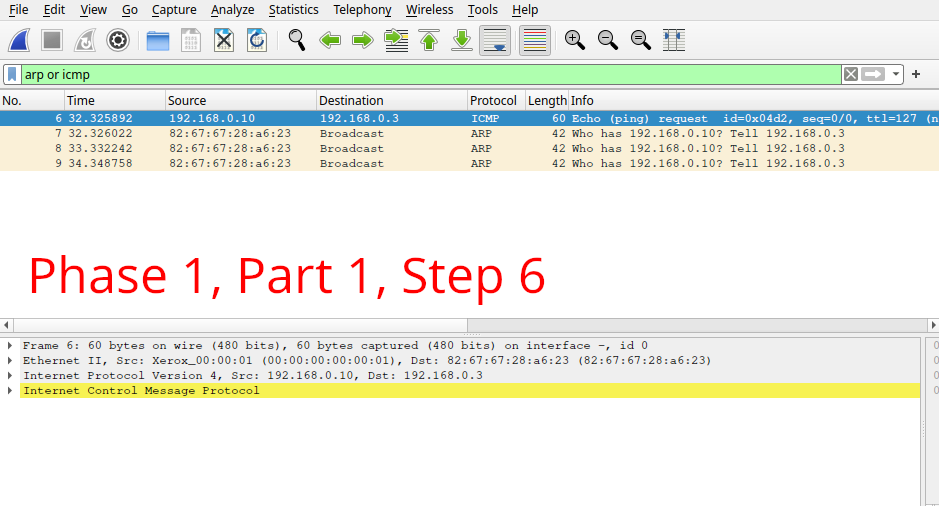
\includegraphics[width=14cm]{data/q5-capture1.png}
		\caption{The Wireshark capture for phase 1, part 1, step 6.}
		\label{fig:wireshark-capture1-q5}
	\end{figure}
	
	\begin{figure}[H]
		\centering
		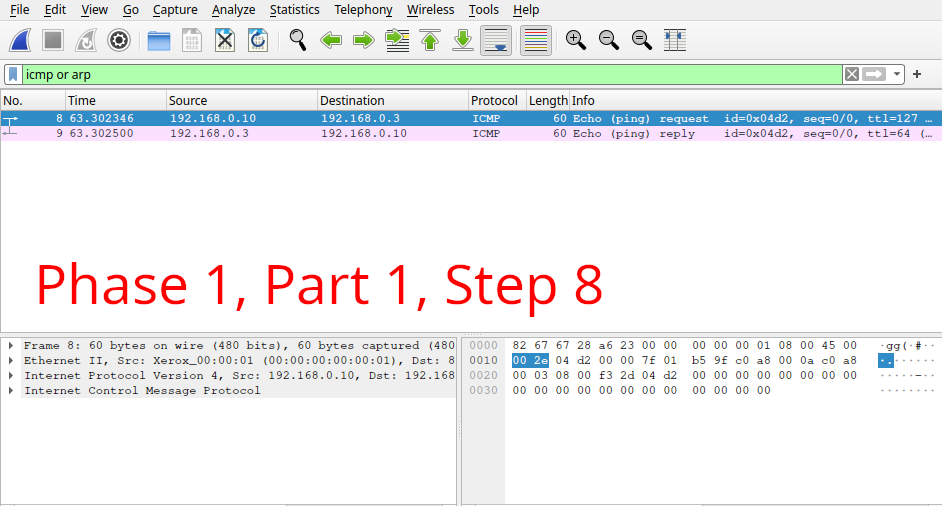
\includegraphics[width=14cm]{data/q5-capture2.png}
		\caption{The Wireshark capture for phase 1, part 1, step 8.}
		\label{fig:wireshark-capture2-q5}
	\end{figure}
	
	\begin{figure}[H]
		\centering
		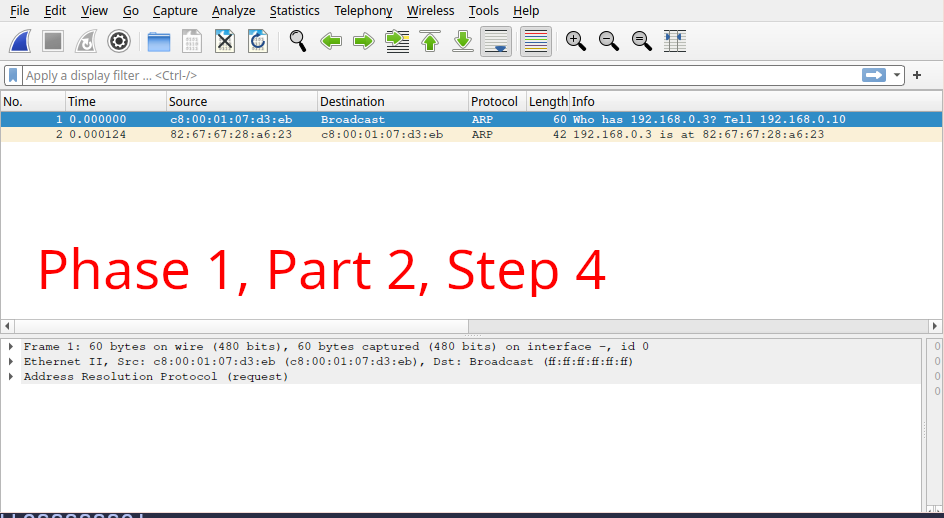
\includegraphics[width=14cm]{data/q5-capture3.png}
		\caption{The Wireshark capture for phase 1, part 2, step 4.}
		\label{fig:wireshark-capture3-q5}
	\end{figure}
	
	\begin{figure}[H]
		\centering
		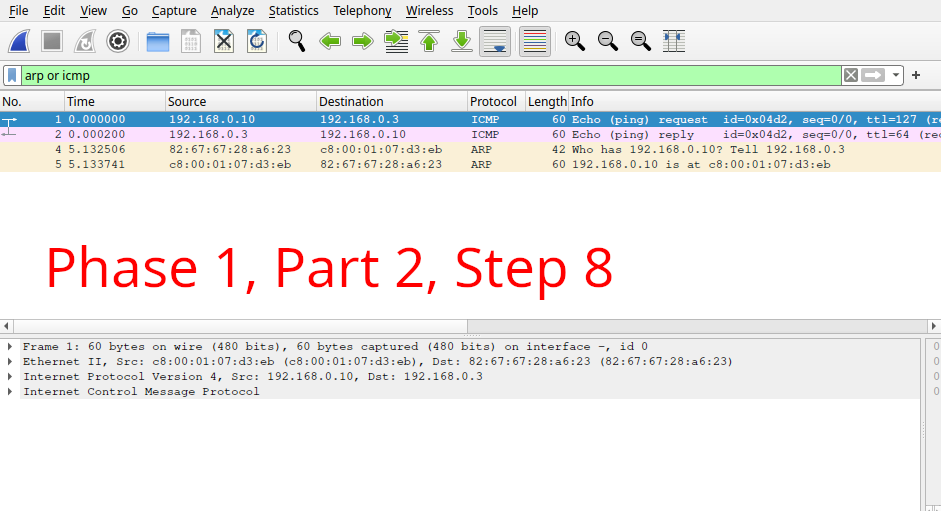
\includegraphics[width=14cm]{data/q5-capture4.png}
		\caption{The Wireshark capture for phase 1, part 2, step 8.}
		\label{fig:wireshark-capture4-q5}
	\end{figure}
	
	The above four pictures are all the Wireshark captures as
	specified in the lab sheet.
	
	All we have to do is notice that the addresses in use are
	From Figure \ref{fig:wireshark-capture1-q5} it can be deduced
	that \texttt{192.168.0.10} and \texttt{192.168.0.3} are the IP
	addresses in use. These are the IP address of the virtual Ostinato
	device and alpine-3 respectively.
	
	
	\begin{note}
		All the captures in Figures \ref{fig:wireshark-capture1-q5},
		\ref{fig:wireshark-capture2-q5}, \ref{fig:wireshark-capture3-q5}
		\& \ref{fig:wireshark-capture4-q5} were made over Hub1 $\leftrightarrow$
		alpine-1. This exposes the nature of hubs as networking devices.
		Hubs do not keep track of any form source and destination. Hubs
		take a broad stroke approach and replay any communication they
		receive into all of their connections.
	\end{note}
\end{ans}

\Que{6}{Compare the packet(s) you capture on Switch1
$\leftrightarrow$ alpine-2. State at least one difference
between your output and that shown in Fig. 37, and explain it.}

\begin{ans}
	For this question all the steps described in
	Phase 1, Part 2 were repeated. However, this time Port 1
	(in Ostinato) was used and connections Switch1 $\leftrightarrow$
	apline-2 and Swtich1 $\leftrightarrow$ apline-4 were monitored.
	
	\begin{figure}[H]
		\centering
		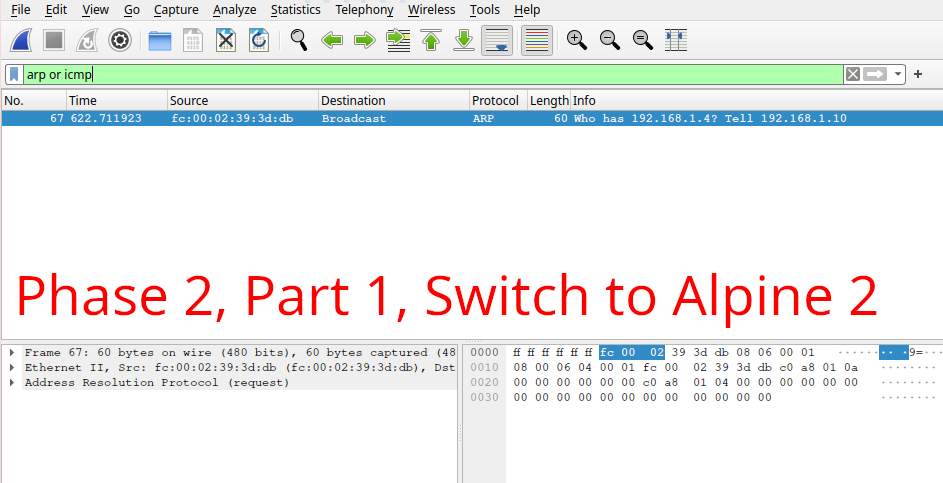
\includegraphics[width=14cm]{data/q6-phase2-switch-to-alpine2-part1.pngg}
		\caption{The Wireshark capture for phase 2, part 1.}
		\label{fig:wireshark-capture4-q5}
	\end{figure}
	
	![Switch to Apline 2 Part 1 for Question 6](data/q6-phase2-switch-to-alpine2-part1.png)
	
	![Switch to Apline 2 Part 2 for Question 6](data/q6-phase2-switch-to-alpine2-part2.png)
	
	Firstly, it is important to note that we only actually capture a
	single packet on the Switch <-> Apline 2 connection as clearly
	established by the pictures above, specifically Switch to Apline
	2 Part 1 and Swithc to Apline 2 Part 2.
	
	Additionally, the only difference between my output and that
	present in Fig. 37 of the lab sheet is the MAC address. However,
	this could have also been made the same since the MAC address
	can be set by the user of Ostinato.
\end{ans}


\Que{7.1}{Present a screenshot that shows the packets you have
captured on Switch1 $\leftrightarrow$ alpine-4.}
% \Ans{Hello}


\Que{7.2}{For each packet, explain how it fits into the sequence that is generated as a result of running the
packet stream you have configured on Ostinato.}
% \Ans{Hello}

\Que{7.3}{Select the ICMP packet generated by Ostinato. Use a
   tabular structure, exemplified by Fig. 39, to name
   \textbf{all} the fields, for all the layers, in the ICMP
   packet. For each field name, write a prefix to indicate which
layer the field pertains to, e.g., L1 for layer 1, L2 for layer
2, etc.}
% \Ans{Hello}

\Que{8}{Explain why the packets captured on Switch1
   $\leftrightarrow$ alpine-2 do not change between the point in
   time just before running the packet stream on Ostinato, and
   the point in time just after
running it.}
% \Ans{Hello}

\Que{9}{
This concerns the dynamics of transmission using TCP. For each
of the four cases (lossless, and packet loss at the rate of 1\%,
3\% and 5\% respectively):
\begin{enumerate}
\item Plot a 1-s MA of the throughput, and
\item calculate the average throughput
\end{enumerate}}
% \Ans{Hello}

\Que{10}{
Consider the packet sequence pertaining to the lossless case.
\begin{enumerate}
\item List the flags (within square brackets) pertaining to the
   first three packets.
\item What part of connection establishment do the first three
   packets pertain to?
\item List the sequence (Seq=) and acknowledgement (Ack=)
   numbers pertaining to the first three packets.
\item Identify the maximum segment size which the two parties in
   the connection state.
\item Identify the range of packets involved in the data
   transfer phase.
\item Identify the packet(s) involved in the connection teardown
   phase.
\end{enumerate}

\textbf{Show screenshots that allow a reader to validate your answers.}}

% \Ans{Hello}

\Que{11}{
Consider the packet sequence pertaining to the 5\% packet loss
case. List \texttt{received\_file} on alpine-4 and compare its
size with that of \texttt{large\_file}.

\textbf{Show screenshots that allow a reader to validate your
answers.}}
% \Ans{Hello}

\Que{12}{
Consider the packet sequence pertaining to the lossless case.
\begin{enumerate}
\item List \texttt{received\_file} on alpine-4 and compare its
   size with that of \\ \texttt{large\_file}.
\item Go to File->Export Packet Dissections, export the captured
   packets as CSV and inspect the CSV file in Excel. How does
   the number of octets sent (as you determine from the CSV
   file) compare with the size of\\ \texttt{received\_file}?
\item Inspect the first few packets in the UDP window and
   identify the length of the UDP datagram (``Len''). How does
   this compare with the Ethernet frame's MTU of 1500? Explain
   any difference you observe.
\end{enumerate}

\textbf{Show screenshots that allow a reader to validate your answers.}}
% \Ans{Hello}

\Que{13}{Explain the difference between your observations in 11
and 12.1.}
% \Ans{Hello}

\end{document}
